\documentclass{article}

\usepackage{amsmath}
\usepackage{graphicx}
\usepackage[a4paper, margin=1in]{geometry}

\begin{document}
	
	\title{Machine Learning Homework: Linear Regression Analysis}
	\author{Vahid Maleki}
	\date{\today}
	\maketitle
	
	\section*{Introduction}
	This document presents the solution to a set of homework questions for the Machine Learning course, specifically focusing on linear regression. Each question includes calculations and, where applicable, visualizations to demonstrate linear regression concepts.
	
	\section*{Question 1: Simple Linear Regression Calculation}
	In this question, we are tasked with calculating the best-fit line for a dataset that includes Weight (as \( x \)) and Systolic Blood Pressure (BP, as \( y \)).
	
	\subsection*{Given Data}
	The dataset includes the following values for Weight and Systolic BP:
	
	\begin{center}
		\begin{tabular}{|c|c|}
			\hline
			Weight (\( x \)) & Systolic BP (\( y \)) \\
			\hline
			165 & 130 \\
			167 & 133 \\
			180 & 150 \\
			\vdots & \vdots \\
			192 & 160 \\
			187 & 159 \\
			\hline
		\end{tabular}
	\end{center}
	
	\subsection*{Step 1: Calculate Means of \( x \) and \( y \)}
	We begin by calculating the mean of \( x \) (Weight) and \( y \) (Systolic BP):
	
	\[
	\bar{x} = \frac{1}{n} \sum_{i=1}^{n} x_i = \frac{165 + 167 + \dots + 187}{26}
	\]
	\[
	\bar{y} = \frac{1}{n} \sum_{i=1}^{n} y_i = \frac{130 + 133 + \dots + 159}{26}
	\]
	
	After performing the calculations:
	\[
	\bar{x} \approx 182.42, \quad \bar{y} \approx 146.31
	\]
	
	\subsection*{Step 2: Calculate the Slope \( m \)}
	The slope \( m \) is calculated as:
	\[
	m = \frac{\sum_{i=1}^{n} (x_i - \bar{x})(y_i - \bar{y})}{\sum_{i=1}^{n} (x_i - \bar{x})^2}
	\]
	
	Calculate each term:
	
	1. \textbf{Calculate \( (x_i - \bar{x})(y_i - \bar{y}) \) and sum them}:
	\[
	\sum_{i=1}^{n} (x_i - \bar{x})(y_i - \bar{y}) \approx 6288.62
	\]
	
	2. \textbf{Calculate \( (x_i - \bar{x})^2 \) and sum them}:
	\[
	\sum_{i=1}^{n} (x_i - \bar{x})^2 \approx 15312.35
	\]
	
	Thus,
	\[
	m = \frac{6288.62}{15312.35} \approx 0.41
	\]
	
	\subsection*{Step 3: Calculate the Intercept \( b \)}
	The intercept \( b \) is given by:
	\[
	b = \bar{y} - m \bar{x}
	\]
	Substitute the values:
	\[
	b = 146.31 - (0.41 \times 182.42) \approx 71.52
	\]
	
	\subsection*{Step 4: Final Equation of the Line}
	The equation of the regression line is:
	\[
	y = mx + b
	\]
	Substitute \( m \) and \( b \) into this equation:
	\[
	y = 0.41x + 71.52
	\]
	
	\subsection*{Visualization}
	\begin{figure}[h!]
		\centering
		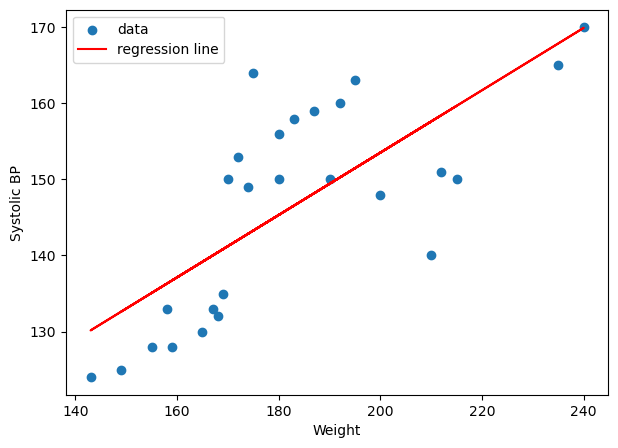
\includegraphics[width=0.6\textwidth]{./images/task1_output.png}
		\caption{Linear regression line fitting the given data points.}
		\label{fig:image1}
	\end{figure}
	
	\newpage
	\section*{Question 2: Multivariate Linear Regression Analysis (30 Marks)}
	This question examines the relationship between wear on a bearing \( y \), oil viscosity \( x_1 \), and load \( x_2 \).
	
	\subsection*{Given Data}
	The dataset includes the following values for oil viscosity (\( x_1 \)), load (\( x_2 \)), and bearing wear (\( y \)):
	
	\begin{center}
		\begin{tabular}{|c|c|c|}
			\hline
			\( x_1 \) & \( x_2 \) & \( y \) \\
			\hline
			1.6 & 851 & 293 \\
			15.5 & 816 & 230 \\
			22.0 & 1058 & 172 \\
			43.0 & 1201 & 91 \\
			33.0 & 1357 & 113 \\
			40.0 & 1115 & 125 \\
			\hline
		\end{tabular}
	\end{center}
	
	
	\subsection*{Part (a): Fit a Multivariate Linear Regression Model (10 Marks)}
	We want to fit a multivariate linear regression model of the form:
	\[
	y = b_0 x_1 + b_1 x_2 + b_2
	\]
	where \( b_0 \), \( b_1 \), and \( b_2 \) are the intercept and coefficients for the variables \( x_1 \) and \( x_2 \), respectively.
	
	We have equation \[XB=Y\] which X is matrix with columns \(x1\) and \(x2\) and we add third column with ones so it's coefficient will be the intercept, B is matrix of intercepts that we must find and Y is matrix with one column y.
	\[
	X=
	\begin{bmatrix}
		1.6 & 851 & 1 \\
		15.5 & 816 & 1 \\
		22.0 & 1058 & 1 \\
		43.0 & 1201 & 1 \\
		33.0 & 1357 & 1 \\
		40.0 & 1115 & 1 \\
	\end{bmatrix}
	\quad B=
	\begin{bmatrix}
		b_0 \\
		b_1 \\
		b_2
	\end{bmatrix} \quad Y=
	\begin{bmatrix}
		293 \\
		230 \\
		172 \\
		91 \\
		113 \\
		125 
	\end{bmatrix}
	\]
	
	But X is not squared mutrix we multiply transpose of matrix \(X\) from right to each side of the equation to create square matrix.(\(X^T X B = X^T Y\))
	
	\[
	\begin{bmatrix}
		5264.8 & 178309.6 & 155.1 \\
		178309.6 & 7036496 & 6398 \\
		155.1 & 6398 & 6.0
	\end{bmatrix}
	\begin{bmatrix}
		b_0 \\
		b_1 \\
		b_2
	\end{bmatrix} =
	\begin{bmatrix}
		20459.8 \\
		1021006 \\
		1024 
	\end{bmatrix}
	\]
	
	now if i convert this matrix to identity matrix the last column will represent the \( b_0 \), \( b_1 \), and \( b_2 \)
	
	
	\[
	\begin{bmatrix}
		5264.8 & 178309.6 & 155.1 & \vert & 20459.8 \\
		178309.6 & 7036496 & 6398 & \vert & 1021006 \\
		155.1 & 6398 & 6.0 & \vert & 1024
	\end{bmatrix}
	\]
	
	and after simplification we end up with this matrix
	
	\[
	\begin{bmatrix}
		1 & 0 & 0 & \vert & -3.8\\
		0 & 1 & 0 & \vert & -0.1\\
		0 & 0 & 1 & \vert & 372.2
	\end{bmatrix}
	\]
	
	\[
	b_0 \approx -3.8, \quad b_1 \approx -0.1, \quad b_2 \approx 372.2
	\]
	
	Thus, the regression model is:
	\[
	y = - 3.8 x_1 - 0.1 x_2 + 372.2
	\]
	
	\subsection*{Visualization} 
	\begin{figure}[h!]
		\centering
		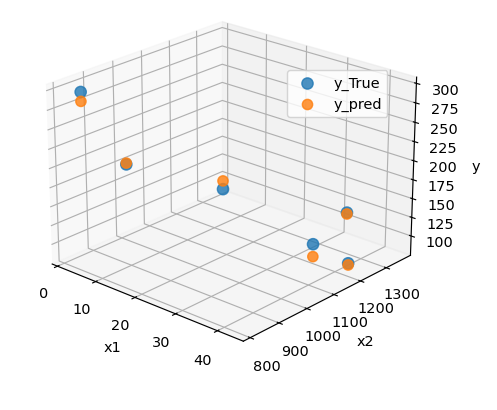
\includegraphics[width=0.6\textwidth]{./images/task2a_output.png}
		\caption{Multivariate Linear Regression}
		\label{fig:image2}
	\end{figure}
	
	
	\section*{Part (b): Predict Wear for \( x_1 = 25 \) and \( x_2 = 1000 \) (5 Marks)}
	To predict the wear \( y \) when \( x_1 = 25 \) and \( x_2 = 1000 \), we substitute these values into our model:
	
	\[
	y = 372.2 - 3.8 \cdot 25 - 0.1 \cdot 1000
	\]
	
	Calculating each term:
	\[
	y = 372.2 - 95 - 100
	\]
	\[
	y \approx 177.2
	\]
	
	Thus, the predicted wear \( y \) when \( x_1 = 25 \) and \( x_2 = 1000 \) is approximately \( 177.2 \).
	
	 \section*{Part (c): Fit a Multivariate Linear Regression Model with Interaction Term \( x_1 x_2 \) (15 Marks)}
	In this part, we add an interaction term \( x_1 x_2 \) to the model. The new model is:
	\[
	y = b_0 + b_1 x_1 + b_2 x_2 + b_3 (x_1 x_2)
	\]
	
	like what we did in part (a) we first calculate \(X\),\(B\) and \(Y\) matrix and solve \(X B = Y\) equation.
	
	this time we add \(x_1 x_2\) as column three of matrix \(X\) and also we add it's coefficient to matrix \(B\)
	
	\[
	X=
	\begin{bmatrix}
		1.6 & 851 & 1361.6 & 1 \\
		15.5 & 816 & 12648 & 1 \\
		22.0 & 1058 & 23276 & 1 \\
		43.0 & 1201 & 51643 & 1 \\
		33.0 & 1357 & 44781 & 1 \\
		40.0 & 1115 & 44600 & 1 \\
	\end{bmatrix}
	\quad B=
	\begin{bmatrix}
		b_0 \\
		b_1 \\
		b_2 \\
		b_3
	\end{bmatrix} \quad Y=
	\begin{bmatrix}
		293 \\
		230 \\
		172 \\
		91 \\
		113 \\
		125 
	\end{bmatrix}
	\]
	
	now just like befor we must multiply the transpose of matrix \(X\) from right to both side of the equation and we end up with this equation
	
	\[
	\begin{bmatrix}
		5264.81 & 178309.6 & 6192716.56 & 155.1 \\
		178309.6 & 7036496 & 208625558 & 6398 \\
		6192716.56 & 208625558 & 7365095440 & 178309.6 \\
		155.1 & 6398 & 178309.6 & 6.0
	\end{bmatrix}
	\begin{bmatrix}
		b_0 \\
		b_1 \\
		b_2 \\
		b_3
	\end{bmatrix}
	\begin{bmatrix}
		20459.8 \\
		1021006 \\
		22646226.8 \\
		1024 
	\end{bmatrix}
	\]
	
	and just like befor we must convert matrix below to identity matrix
	
	\[
	\begin{bmatrix}
		5264.81 & 178309.6 & 6192716.56 & 155.1 & \vert & 20459.8 \\
		178309.6 & 7036496 & 208625558 & 6398 & \vert & 1021006 \\
		6192716.56 & 208625558 & 7365095440 & 178309.6 & \vert & 22646226.8 \\
		155.1 & 6398 & 178309.6 & 6.0 & \vert & 1024
	\end{bmatrix}
	\]
	
	and we end up with this matrix
	
	\[
	\begin{bmatrix}
		1 & 0 & 0 & 0 & \vert & -7.6 \\
		0 & 1 & 0 & 0 & \vert & -0.22 \\
		0 & 0 & 1 & 0 & \vert & 0.004 \\
		0 & 0 & 0 & 1 & \vert & 483.96 \\
	\end{bmatrix}
	\]
	
	\[
	b_0 \approx -7.6, \quad b_1 \approx -0.22, \quad b_2 \approx 0.004 \quad b_3 \approx 483.96
	\]
	
	Thus, the regression model is:
	\[
	y = - 7.6 x_1 - 0.22 x_2 + 0.004 x_1 x_2 + 483.96
	\]
	
	
	\section*{Question 3}
	
	\subsection*{Part (a): Matrix Formulation of \( O = ZW \) (20 Marks)}
	
	The regression model can be expressed in the form \( O = ZW \), where:
	\[
	O = \begin{bmatrix} o_1 \\ o_2 \\ \vdots \\ o_m \end{bmatrix}, \quad 
	W = \begin{bmatrix} w_0 \\ w_1 \\ w_1 \\ w_2 \\ w_2 \\ \vdots \\ w_n \\ w_n \end{bmatrix}
	\]
	
	The matrix \( Z \) is constructed from the input data as follows:
	\[
	Z = \begin{bmatrix}
		1 & x_{1}^{(1)} & \left( x_{1}^{(1)} \right)^3 & x_{2}^{(1)} & \left( x_{2}^{(1)} \right)^3 & \cdots & x_{n}^{(1)} & \left( x_{n}^{(1)} \right)^3 \\
		1 & x_{1}^{(2)} & \left( x_{1}^{(2)} \right)^3 & x_{2}^{(2)} & \left( x_{2}^{(2)} \right)^3 & \cdots & x_{n}^{(2)} & \left( x_{n}^{(2)} \right)^3 \\
		\vdots & \vdots & \vdots & \vdots & \vdots & \cdots & \vdots & \vdots \\
		1 & x_{1}^{(m)} & \left( x_{1}^{(m)} \right)^3 & x_{2}^{(m)} & \left( x_{2}^{(m)} \right)^3 & \cdots & x_{n}^{(m)} & \left( x_{n}^{(m)} \right)^3 \\
	\end{bmatrix}
	\]
	
	Thus, each element in \( O \) is given by:
	\[
	o^{(j)} = w_0 + w_1 x_1^{(j)} + w_1 \left( x_1^{(j)} \right)^3 + w_2 x_2^{(j)} + w_2 \left( x_2^{(j)} \right)^3 + \dots + w_n x_n^{(j)} + w_n \left( x_n^{(j)} \right)^3
	\]
	where \( j = 1, 2, \dots, m \) represents each sample in the dataset.
	
	\subsection*{Part (b): Gradient Descent Update Rule for \( w_i \) (10 Marks)}
	
	To find \( W \) using gradient descent, we update each \( w_i \) according to the following rule:
	\[
	w_i \leftarrow w_i - \eta \frac{\partial}{\partial w_i} \left( \frac{1}{m} \sum_{j=1}^{m} \left( o^{(j)} - \hat{o}^{(j)} \right)^2 \right)
	\]
	where:
	- \( \eta \) is the learning rate,
	- \( o^{(j)} \) is the actual output for sample \( j \),
	- \( \hat{o}^{(j)} = w_0 + w_1 x_1^{(j)} + w_1 \left( x_1^{(j)} \right)^3 + \dots + w_n x_n^{(j)} + w_n \left( x_n^{(j)} \right)^3 \) is the predicted output.
	
	For simplicity, the update rule for each \( w_i \) can be written as:
	\[
	w_i \leftarrow w_i - \eta \cdot \frac{1}{m} \sum_{j=1}^{m} \left( o^{(j)} - \hat{o}^{(j)} \right) \frac{\partial \hat{o}^{(j)}}{\partial w_i}
	\]
	
	\textbf{Note}: The update relation for the bias term \( w_0 \) is not required in this problem.
	
	
	
\end{document}
